\chapter{Problem analysis}
\label{chapter4}
%phd report
%https://roadnighttaylor.co.uk/news/what-is-active-network-management/
%Curtailment + curtailment % + solution/compensations
%https://windeurope.org/wp-content/uploads/files/policy/position-papers/WindEurope-Priority-Dispatch-and-Curtailment.pdf
The principle of active network management \gls{ANM} is to address congestion and voltage issues via short-term decision making policies \cite{ANMQuentin}. \\
\gls{ANM} creates a smarter network infrastructure providing automated control of various components in the network and provides the information needed to ensure that every device performs in an optimal manner. This automated control allows grid companies to avoid the traditional approach of reinforcing the network with expensive upgrades; so reducing the costs.
For example, in case of energy generation from the renewable devices higher than what a particular line can handle, a grid company, to avoid congestions and possible overvoltages, has three main options:
\begin{itemize}
    \item Replace the existing line with a line that can handle a higher voltage. This usually means to replace the existing line with a cable with a larger cross-sectional area.
    \item Add another parallel line.
    \item Handle the situation with \gls{ANM}.
\end{itemize}
The first two solutions require some infrastructure investment that can be expensive and troublesome, especially in the case of overhead or underground lines.\\
The solution with \gls{ANM} does not require construction cost for the grid company; to keep the network working, in this case, the output of the renewable devices can be curtailed to reduce lines' overloading. \\

In these references, generally, \gls{ANM} maintains the system within operational limits by relying on the curtailment of the generator devices, \glspl{PV}, \glspl{WP} and other \gls{DER} devices. \\
Curtailment of renewable energy may be seen as counter-intuitive on the environmental point of view, and it may be considered as last option. Indeed, this process can slow down the switch to clean energy, because of the lost of the curtailed energy. \\

In this mindset, \gls{ANM} could also be used to control flexible loads and reduce the curtailment effects. These flexible loads, also known as virtual batteries, such as water heaters, air conditioning systems, electric vehicles, can be controlled to be turned on if the energy production is higher than the energy consumption so to avoid curtailment on the generators \cite{flexibleloads}. \\
Another way to reduce the energy curtailment is to use Flexible Alternating Current Transmission System (\gls{FACTS}) devices. They offer some
level of power flow control and enhance the transfer capability over the existing network. This flexibility can be utilized for congestion
mitigation and renewable energy integration. Particularly, \gls{FACTS} devices allow controlling all parameters that determine active and reactive power transmission: nodal voltages magnitudes and angles and line reactance. These devices replace the mechanical switches with semiconductor switches allowed much faster response times. One problem with these devices is the cost a system operator should sustain to implement them in the network \cite{facts}.


\section{Network topology}
\label{sec:nt}
A power network can be represented as a direct graph $\mathcal{G}(\mathcal{N},\mathcal{E})$, where \gls{N} is a set of nodes, also called buses in the network, \gls{E} $\subseteq \mathcal{N} \times \mathcal{N}$ is the set of directed edges linking two buses together, also called lines. The notation \gls{e} $\in \mathcal{E}$ refers to the directed edge with sending bus $i$ and receiving bus $j$. Each bus might be connected to several devices, which may inject or withdraw power from the grid. The set of all devices is denoted by \gls{D} that can be either loads \gls{L} or generators \gls{G}. \\
Power networks generally operate radially as a tree, with the root the substation. The root substation can be seen as a slack bus, where the voltage magnitude \gls{V} and the phase angle \gls{angleV} are considered constants.
% Several variables are associated with each bus $n \in \mathcal{N}$: a bus voltage $\mathcal{V}_i$, a bus current injection $I_i$, an active power injection $P_i$ and reactive power injection $Q_i$. 
%The complex powers $S_i$, $S_d$ $\in \mathbb{C}$ injected into the network at bus $i$, or device $d$, can be obtained by the relation $S_i = P_i + \mathbf{i}Q_i$ or $S_d = P_d + \mathbf{i}Q_d$. \\
%Similarly, variables $I_{ij}$, $P_{ij}$, $Q_{ij}$ and $S_{ij}$ refer to the direct flow of the quantities in branch $e_{ij}$ as measured at bus $i$ \cite{gym-anm}.\\

\section{Problem statement}
\label{sec:ps}
This thesis will focus on \gsl{ANM} and the problem faced by a \gsl{DSO} to maintain the network within its operational limits. In particular, the system operator will evaluate whether in a given moment there will be a voltage problem, so that it would be possible to proceed with some actions, like applying curtailment to generator devices, to maintain the voltage inside a safe range.\\

The \gls{DSO} knows some information about the network:
\begin{itemize}
    \item The network topology: the number of buses, loads and generators, the lines' length, the distance between the connected buses, and the distance between each load and generator from the external grid. Moreover, the impedance of the lines is known.
    
    \item The active and reactive power of some loads at each time step. Some values may not available mainly for two reasons: \emph{a)} for that particular load there are no measurements at all due to privacy reasons or for the lack of sensors or \emph{b)} communication problem so the sensor recording was lost. \emph{remove?}
    
    \item The type of \gsl{DER} device connected to each bus. If the \gls{DER} device is directly connected to the medium voltage grid, the active power and reactive power are considered known. 
\end{itemize}

This data is used to calculate the power flow of the network and obtain more information like the voltage magnitude at each bus, lines' loading and other values. This calculation can be performed with any power system analysis tool, for this thesis Pandapower will be used.\\

%Moreover, since the power flow depends on the power injection of the different elements, it is possible to create some possible cases changing the active and reactive power of the devices. These cases can be generated multiplying the time series by some scaling factors to increase or decrease the injection values.  \\

%https://arxiv.org/ftp/arxiv/papers/2102/2102.05657.pdf
The \gls{DSO} will consider the behaviour of the network over a set of discrete time steps $t \in \{1,2,...,T-1,T\}$ of length $\Delta t$, with, $T \in \mathbb{N}$, the last time step of the time series’ horizon. A time step is considered as a snapshot of the system at one particular point in time. \\ 

The \gls{DSO} can have access to some information, let's define the information domain as $\textbf{I}$. This information can be divided in static information like the network topology, and the observation $O_t$ collected at every time step $t$ like the loads and generators' active and reactive power and the buses' voltage magnitude and lines' loading. The information at time step $I_t$ can be defined as:
\begin{align*}
    I_t & \in \textbf{I}, \text{with} \, t \in \{1,2,...,T-1,T\} \\
    I_t & = \langle\text{static information}, O_1, O_2, ...\rangle
\end{align*}
\noindent In general power networks are not static, since the operators can modify their topology, for example changing the connections due to some incidents on the lines. In this thesis, the network topology is considered as static, so that no changes are applied on the network the during the whole time series' horizon.\\

\noindent An instance of the observation $O_i$ can be:
\begin{equation*}
    O_i = \langle P\,^{load}_{l,i}, Q\,^{load}_{l,i}, P\,^{sgen}_{g,i}, V^{bus}_{v,i}, I^{line}_{\%}\,_{e,i} \rangle
\end{equation*}
\noindent where $P\,^{load}_{l,i}$ and $Q\,^{load}_{l,i}$ are active and reactive power of load $l$ at time stamp $i$, with $l \in \{0, ..., |\mathcal{L}|\}$ and $|\mathcal{L}|$ the total number of loads in the network; 
$P\,^{sgen}_{g,i}$ is the active power of the generator $g$ at time $t$, with $g \in \{0, ..., |\mathcal{G}|\}$ and $|\mathcal{G}|$ the total number of generators; 
$V^{bus}_{b,i}$ is the voltage magnitude (in \gls{pu}) of the bus $b$ at time $t$, with $b \in \{0, ..., |\mathcal{N}|\}$ and $|\mathcal{N}|$ the total number of buses (or nodes);
$I^{line}_{\%}\,_{e,i}$ is the line loading (in $\%$) of the line $e$ at time $t$, with $e \in \{0, ..., |\mathcal{E}|\}$ and $|\mathcal{E}|$ the total number of lines (or edges)
.\\

The operator will predict if the system, in some given $t+n$ future time steps, will be in a critical condition. The network is considered in a critical condition if any of its elements is in an unsafe situation, for example an over voltage condition. Let define $\textbf{C}$ as the list of critical situation and $C_t$ the critical situation at time step $t$, with $C_t \in \{0,1\}$.  \\
For predicting whether the system will be in a critical situation or not, the \gls{DSO} will consider the history of the system only for $h$ preceding steps, with $h \in \mathbb{N}^+$. \\

Let also define the function $f_\mathcal{N}$ that given the information from a particular network can elaborate this information and output some values, that represent the forecasting of a critical situation. \\
It is possible to summarize all the information under the relationship:
\begin{equation} \label{eq:fmapping}
    %C = f_\mathcal{N}(I_{t-h+1},I_{t-h+2},\dots,I_{t-1},I_{t})
    \hat{\textbf{C}} = f_\mathcal{N}(\textbf{I})
\end{equation}
\noindent where $\hat{\textbf{C}}$ represents the forecasted values of the system given the information $\textbf{I}$. A single instance $\hat{C}_{t+i}$ ($\hat{C}_{t+i} \in \{0,1\}$) states if the system is critical ($\hat{C}_{t+i}=1$) or not ($\hat{C}_{t+i}=0$), with $i \in \{1,2,\dots,n-1,n\}$ and $n \in \mathbb{N}^+$. \\

% \begin{itemize}
    % \item $\textbf{I}$ is the information domain about the network. %and $I_i$ is the information vector, with $I \in \textbf{I}$, of the system at one generic time step $i$.
    % $\textbf{I}$ represent some information like the network topology, the loads and generators' active and reactive power and the buses' voltage magnitude, lines' loading and other information.
    
    % \item $h$ is the number of how many history time steps will be considered. $h \in \mathbb{N}^+$.
    
    % \item $f_\mathcal{N}$ is a generic function that maps the input information of the system to the critical system evaluation, and the subscript $\mathcal{N}$ refers to the fact that the function depends on the particular network considered. \\
    % Henceforth, the function will be referenced without the $\mathcal{N}$ subscript.% $P: \mathbb{R}^{h,n} \mapsto \{0,1\}^f$.
    
%     \item $\hat{\textbf{C}}$ represents the forecasted values of the system given the information $\textbf{I}$. A single instance $\hat{C}_{t+i}$ ($\hat{C}_{t+i} \in \{0,1\}$) states if the system is critical ($\hat{C}_{t+i}=1$) or not ($\hat{C}_{t+i}=0$), with $i \in \{1,2,\dots,n-1,n\}$ and $n \in \mathbb{N}^+$. 
%     %The network is considered in a critical situation when the following condition holds
% \end{itemize}

The main objective is to find a good mapping function $f_\mathcal{N}$ such that the actual critical values $\textbf{C}$ and forecasted values $\hat{\textbf{C}}$ are as close as possible.

\section{Solving methodology}
\label{sec:sm}
The goal of this thesis is to find a practical function $f_\mathcal{N}$. This function, that can be considered as a pipeline, mainly consist of some steps:
\begin{itemize}
    \item Solve the partial-observability problem, generating realistic time series or filling the missing measurements for the different elements. These time series are needed to run the power flow calculation. \emph{Remove?}
    \item Process the information to build a dataset, consisting of $\{\textbf{x,y}\}$ couples given by the information of the network $\textbf{I}$ and the critical states $\textbf{C}$.
    \item Use the generated dataset to train a classifier that can forecast whether the network will be in a critical situation.
\end{itemize}

\subsection{Partial-observability problem}
%https://arxiv.org/pdf/2108.08350.pdf
As mentioned, the network has only a partial-observability mainly due to \emph{a)} values not available at all or \emph{b)} few missing values. \\

Missing values problems can be solved filling these measurements with some techniques: balancing the flow of the network or using generative models in the case of \emph{a)} or using the values from the adjacent time steps, averages or more complex methods like for example interpolation in the case of \emph{b)}. \\

These methods will allow complementing the network time series and having sufficient data to perform the power flow calculation.

\subsection{Processing}
Given all the information about the network, only a subset will be used to train the classifier, in particular the information given from the power flow calculation, that can be the voltage magnitude at each bus or the lines' loading. \\

This subset of information is divided in windows of length $h$ for the history time series, that correspond to the inputs $\textbf{x}$s and in outputs $\textbf{y}$s, of length $n$ of future time steps, that correspond to the labels.

% \begin{equation*}
%     \textbf{x} & \subseteq \textbf{I}
% \end{equation*}

% \begin{equation*}
%     \begin{aligned}
%         \textbf{y} & = C \\
%     & = [C_{t+1},C_{t+2}, \dots, C_{t+f-1},C_{t+f}]
%     \end{aligned}
% \end{equation*}
%In particular, the \gls{ANN} inputs consist of state variables from time instance $t-h+1$ to $t$. According to \ref{eq:fmapping} and \ref{eq:systemState}, the input can be expressed as a matrix of state variable:

\subsection{Forecasting}
It is common in time series forecasting problems to use artificial neural networks (\glspl{ANN}) to find a solution, thanks to their capacity to learn an approximate mapping function from the input space to the output space. In this case, the \gls{ANN} will take as input the information from the network, and it will output binary values, stating if there will be or not a critical situation in the network. \\

\noindent Given the input $\textbf{x}$, the \gls{ANN} must output some binary values stating whether the system is safe or in a critical situation at the time steps $t+n$. \\

This database, given by the couple of elements \{\textbf{x,y}\}, will be used with supervised learning techniques that may extract a forecasting function in order to solve the problem. \\

%The dataset will be split in train, validation and test set in order to train and validate the \gls{ANN}.

% \section{Problem statement}
% \label{sec:ProbStat}
% [\emph{old}] With the increasing number of renewable energy generators entering the power distribution systems, more and more stress is placed on the networks. This energy produced by the generators can increase the voltage in certain points of the network, causing blackouts or damaging the network's transmission lines. These are interruptions of the energy distribution, and they must be avoided. \\

% A possible solution to this problem is to control the renewable energy generators to produce less than what they could have produced; known as curtailment process. \\
% In a distribution network, there are some information for the elements connected to the grid, like active and reactive power, magnitude voltage value and so on. These values are recorded and expressed as a multi-dimentional time series.\\

% More formally, given the directed graph \gls{G}, at timestamp $t$ it is possible to know the feature $X=[l_p,l_q,b_V,e_L]$ with $l_p$ and $l_q$ are the active and reactive power of each load $l \in \mathcal{L}$, $b_V$ are the buses voltage and $e_L$ are the loadings of the edge connecting 2 buses. It is possible that $X$ is known, or only a subset of it, $X_s \subset X$ is known due to non-fully observability of the network. This $X$ time series dataset will be the input of an artificial neural network \gsl{ANN}.\\
% The problem can be solved as a classification or regression problem: 
% \begin{itemize}
%     \item as a classification problem, the output of the \gsl{ANN} will be a binary value that states if in the next $n$ time steps there will be an over or under voltage problem. For the loss, many loss functions can be used, for example a binary cross-entropy loss function. Given $p(y_i) \in \{0,1\}$ the output probability prediction given the input $x \in X$ (or $x_c \in X_c$) the loss would be calculated as follows: 
%     \[
%     H = - \frac{1}{N} \sum_{i=1}^{N} y_i \log{(p(y_i))} + (1 - y_i) \log{(1 - p(y_i))} 
%     \]
%     where $y_i$ is the real label, $p(y_i)$ is the predicted probability that there will be a voltage problem and N is the number of inputs.
%     \item for the regression problem, the output of the \gls{ANN} will be the voltage forecast for each buses for the next $n$ time steps. Also for this problem, many loss functions can be used, for example a \gls{MAE} loss function, calculated as follows:
%     \[
%     MAE = \frac{1}{T \cdot N} \sum_{t=1}^{T} \sum_{i=1}^{N} |y_{t,i} - \hat{y}_{t,i}|
%     \]
%     where $y_{t,i}$ is the real voltage value at time $t$, $\hat{y}_{t,i}$ is the predicted voltage at time $t$ and $T$ is the number of future time steps to forecast.
% \end{itemize}

% The distribution network used is the MV Oberrhein network from Pandapower and the time series are taken from the Simbench dataset. This database refers to some real distribution networks in Germany in the year 2016; the dataset spans over one year with a $\Delta t$ of 15 minutes (a total of 35,040 time steps).

% \section{Optimization problem}
% This voltage control problem can be formulated as a stochastic problem, where the goal is to minimise the losses while meeting some constraints. In particular, the objective is to minimise the loss $L_g$ of each generator $g \in$ \gls{G} due to the curtailment and avoid not useful transport of energy and other minor energy losses $L_{\epsilon}$ (read: L of epsilon). Moreover, the system has to satisfy the condition of loads demands, that the network is considered safe and the congestion risk of each edge $r_{e_{ij}}$ is less than a given maximum tolerated congestion risk $R_{e_{ij}}$, e.g. {1\%} and that the power generated by each generator $\bar{g}_p$ is less or equal to its maximum installed capacity $g^{max}_p$, and the active and reactive power of the loads ($\bar{l}_p$, $\bar{l}_q$) are in their limits. \\
% Mathematically (\cite{haulogypaper}):
% \[
% min \sum_{g \in G} L_g + L_{\epsilon}
% \]
% subject to
% \begin{equation*}
% \begin{aligned}
% & r_{e_{ij}} < R_{e_{ij}} \qquad & \forall e \in \mathcal{E} \\
% & g^{min}_p \leq \bar{g}_p \leq g^{max}_p \qquad & \forall g \in \mathcal{G} \\
% & l^{min}_p \leq \bar{l}_p \leq l^{max}_p \qquad & \forall l \in \mathcal{L} \\
% & l^{min}_q \leq \bar{l}_q \leq l^{max}_q \qquad & \forall l \in \mathcal{L} \\
% \end{aligned}
% \end{equation*}


\section{Reinforcement learning}
\label{sec:rl}
\subsection{Literature review}
Brief literature review for RL application on power networks (paper's link in the titles): \\

\begin{itemize}
    \item \href{https://ietresearch.onlinelibrary.wiley.com/doi/epdf/10.1049/iet-stg.2019.0196}{\textbf{Reinforcement learning for control of flexibility providers in a residential microgrid}}\\
    
    A multiagent setting, two RL agents – battery agent and HP (heat pump) agent are considered to control the operation of the battery and HP.\\
    Small ‘micro grid’ (<10 devices)\\
    
    HP agent: The goal of the heat pump agent is to maximize self-consumption and to minimise the electricity cost while maintaining the indoor temperature within the comfort boundaries chosen by the end user.\\
    Battery agent: The battery agent controls the operation of the battery to ensure that all the power not consumed by the baseload and/or the HP is stored in the battery. Also, in situations of high electricity prices and low PV generation, the battery agent discharges the battery to match the load.\\
    
    \textbf{State}: different for battery and HP (and for single or multiagent) but basically they use active power for gens (PV), the active power of the load, and the cost for buying electricity.\\
    \textbf{Action}: (discrete) charge/discharge devices\\
    \textbf{Cost function} ∝ energy produced x energy cost (production) + energy used x energy cost (consumption)\\
    \textbf{Models}: Q-network\\
    
    \item \href
    {https://ieeexplore.ieee.org/document/9399637}
    {\textbf{Data-Driven Multi-Agent Deep Reinforcement Learning for Distribution System Decentralized Voltage Control With High Penetration of PVs}}\\
    
    The proposed multiagent deep reinforcement learning (MADRL) can coordinate both the real and reactive power control of PVs with existing static var compensators and battery storage system (BSS) to minimize the voltage deviation while maintaining a minimum amount of active power curtailment of PVs Action each agent represents a subnetwork.(342-node systems)\\
    
    \textbf{State}: active and reactive power of loads, active power of the generators. \\
    \textbf{Action}: not well defined\\
    \textbf{Reward}: voltage fluctuation + curtailed energy\\
    \textbf{Models}: SAC and MATD3 \\
    \textbf{Training}: trained for 50000 episodes. Exploration first 1000 episode.

    
    \item \href
    {https://arxiv.org/abs/2103.07932}
    {\textbf{Gym-ANM: Reinforcement Learning Environments for Active Network Management Tasks in Electricity Distribution Systems}}\\
    We seek to promote the application of RL techniques to active network management (ANM) problems, to design a control schemes that modulate the generators, the loads, and/or the DES devices connected to the grid. This is done to avoid problems at the distribution level and maximize profitability through, e.g., avoidable energy loss.\\
    \\\textbf{State}: p and q loads, max production of gens
    \\\textbf{Action}: a value between the bottom and upper limit on the active and reactive power injection for each generator g. The action space is normalized in [-1,1](?)
    \\\textbf{Reward}: power loss at each instant + penalty term for violation of constraints (line loading, bus voltage, ...)
    \\\textbf{Models}: PPO (Proximal Policy Optimization), SAC (Soft Actor-Critic) both with a continuos action space\\
    
    I like the reward function, I am not sure about the action space.
    
    
    \item \href
    {https://arxiv.org/pdf/1910.05907.pdf}
    {\textbf{Coordination of PV Smart Inverters Using Deep Reinforcement Learning for Grid Voltage Regulation}}\\
    a deep reinforcement learning (DRL) based algorithm is developed and implemented for coordinating multiple SIs to ensure voltage operation limits of the grid are meet. (37 node test feeder)\\
    
    \emph{"The other objective is to minimize the PV production curtailment, which is assured by minimization of reactive power utilization." \\
    Could you clarify the relationship between curtailment and reactive power?\\
    } \\
    
    \\\textbf{State}: voltage magnitudes of each bus, real and reactive power of PVs and loads
    \\\textbf{Action}: we consider SI (smart inverter) reactive power outputs as actions
    \\\textbf{Reward}:the objectives are mitigation of voltage violations and minimization of PV generation curtailment. A large penalty for violating voltage limits and a negative reward proportional to total reactive power dispatched by SIs.
    \\\textbf{Models}: deep deterministic policy gradient (DDPG)
    \\\textbf{Training}: 1500 episodes, each of 1000 iterations
    \\Nice results
    
    \item \href
    {https://www.researchgate.net/publication/341779029_A_Multi-Agent_Deep_Reinforcement_Learning_Based_Voltage_Regulation_Using_Coordinated_PV_Inverters}
    {\textbf{A Multi-Agent Deep Reinforcement Learning Based Voltage Regulation Using Coordinated PV Inverters}}\\ 
    This paper proposes a multi-agent deep reinforcement learning-based approach (MADRL) for distribution system voltage regulation with high penetration of photovoltaics (PV). (33-bus system, and 123-bus system)\\
    
    
    \\\textbf{State}: active and reactive power of loads and active power of gens(PV)
    \\\textbf{Action}: reactive power gens
    \\\textbf{Reward}: voltage deviation (?)
    \\\textbf{Models}: deep deterministic policy gradient (DDPG)
    \\\textbf{Training}: 14000 episodes, each of 24 iterations (hourly). Exploration first 2000 ep
\end{itemize}


\subsection{My proposal}
Using RL to control the gens (PV and WP) active power output.\\

\noindent \textbf{State}: active and reactive power of loads and active power of gens at time step $t$ OR from time step $t-h+1$ to time step $t$ ($h$ time steps). \\
\[
s_t = [P_{load,t},Q_{load,t},P_{gen,t}] \cdot h
\]
\noindent this state would be a list of continuos variables of size 182 x h (61 + 61 + 60); with $h=4$ (consider only 1 h network history) the dimension of the state space would be 728 continuous variables.\\

\noindent\textbf{Action}: the curtailment of the active power of each generator at time $t+1$ in percentage
\[
a_t = [P^{cur\%}_{load,t}]
\]
\noindent this state would be a list of continuos variables of size 60 (call it |A|). \\
OR \\
The same as above, but with one more boolean variable that indicates whether in the next time step ($t+1$) there will be a critical situation. "Double stream network"\\

In the last case, the problem would be both a regression and classification problem. The results can be compared with the work I have already done on the classification part, if the results are similar that would solve two problems with a single model.\\
I think it is an interesting idea also because I have not found many RL problems with a classification and regression problem. \\

There are few problems I can think about: 1) RL algorithms for classification are slower and perform worse than similar models trained with standard supervised learning; 2) so it may not converge; 3) a custom model should be built that it may not be a problem.\\

For the regression problem I am not sure about the range of the action space: should it be [0,1] (it means that there are no constraints and that we can handle a 100\% energy loss, as long as the network is safe), [0,0.1] (we want a curtailment less than 10\% of the total production) or other values? A possible problem may be that even if the actor decides to curtail, in a given time step, many generators, by a large value the network may still be in a critical situation. \\

So the question:\\
\emph{Q: How much can generators be curtailed? \\ "For example, PSCO has reported periods of very high levels of wind generation relative to total demand and has curtailed on the order of 1\%–2\% of wind generation annually in recent years. ...  Curtailment levels have generally been 4\% or less of wind energy generation in regions where curtailment has occurred." \href{https://www.nrel.gov/docs/fy14osti/60983.pdf}{[ref]}) }\\

\noindent \textbf{Reward}: 
Since it is important it may be defined better while proceeding, but here is a possible implementation:
\[
r_t(s,a) = - \alpha \cdot \mathtext{total\_perc\_loss} - \beta \cdot \mathtext{network\_violations} = -
\alpha \cdot \sum^{|A|}_{i=0} a_i + \beta \cdot \phi(s,a)
\]
\noindent where $r_t(s,a)$ is the reward at time $t$ given the state $s$ and action $a$; $\mathtext{total\_perc\_loss}$ is the percentage of energy lost in that time step (sum of all curtailed values, basically np.sum($a_t$)); $\mathtext{network\_violations}$ is a violation term to punish the agent if the network is in a critical situation (voltage above the limit, line loading above the limit, ...); $\alpha$ and $\beta$ are two scaling factors. In case of the double stream network, the classification variable can be used in the reward function as well; something like "$- \gamma \cdot |y_t - \hat{y}_t|$", with $y_t$ the prediction of the model and $\hat{y}_t$ the actual label (known from the power flow calculation) and $\gamma$ another scaling factor.\\

I am not sure with this reward function the agent may converge because is not very specific and does not punish the agent correctly. Maybe it would help to have a $\hat{a}_t$ so to compare with $a_t$ but maybe this is not feasible, and it looks a lot like a supervised problem(?).\\
So the question:\\
\emph{Q: Is there a way (droop-based method? \href{https://par.nsf.gov/servlets/purl/10082801}{[ref]}) to analytically calculate the active and reactive power of loads and generators to avoid overvoltage problems? \\
This would also allow shaping a better reward function and improve convergence}\\

\noindent \textbf{Model}: not sure for now, both state and action are continuos so a model that can handle this kind of values must be needed, so some actor-critic method (PPO, DDPG)\\

\noindent \textbf{Training}: some episode, with each episode given all the time steps\\

\noindent \textbf{General thoughts}: given the time series for p and q of the loads and p of the generators, the power flow can be calculated and the buses' voltage and can be used to check whether the agent (after training) improved the network situation (the number of critical situation decreased). \\

The dataset can be divided in training and test set: the training can be used for each episode; it would work also a data augmentation since at each episode the agent would pick a different action (with high probability) so increasing the size of the dataset; the test set can be used at the end of each episode to test the model and evaluate its performances. \\

There should not be too many problems using the models already implemented: MLP, CNN, and RNN.\\

Probably the pandapower core library should be changed to have a custom control of the time series execution. This should not be a problem since pandapower is open source and the code is available on GitHub. \\

\noindent \textbf{Possible problems:}
\begin{enumerate}
    \item Too high state space (curse of dimensionality)
    \item Action space should be better defined.\\
    Trying running a PF with a reduced energy production by 5\% of all gens reduced the critical situation by 0.8\% (from 3.8\% to 3\%); so maybe it is not the right direction (?)
    \item No converging model, for some reasons: not accurate reward function, too much time required
    \item Messing up with pandapower code and obtaining wrong results
    \item Computationally expensive
    \item Remaining time may not be enough
\end{enumerate}

\noindent \textbf{Updates:}
\begin{enumerate}
    \item I tried to implement the code needed (both change Pandapower code and implementing the DDPG agent code)
    \item the code looks like it is working fine
    \item The training time seems not too bad: it takes 3 more time (around 1 h) than a normal run; with a MLP with 2 hidden layers with 400 and 300 neurons, trained every 2 time steps.\\
    It takes 39 mins for training (70\% of all time series, repeated for 2 episodes) and 9 mins for testing (the remaining 30\% of the time series)
    \item I tested a simple reward function:
    \begin{align*}
        r = &- alpha * np.sum(action) \\
            &- beta*[|1.05-np.max(vm\_pus)|+\frac{1}{2}*|0.95-np.min(vm\_pus)|]^2
    \end{align*}
    with alpha=1, beta=500 (the difference between voltage is quite small), action is the list of res curtailment values([0,100\%]), vm\_pus is the list buses' voltage magnitude after the PF calculation. The idea to punish the agent to curtail too much the generation (np.sum(action)) and punish it if the voltage is out of the constraints. It did not work well. \\
    
    Tested another one:
    \begin{align*}
        r = &- alpha * np.sum(action) \\
            &- \sum_{v \in vm\_pus} f(v)
    \end{align*}
    with f() a piecewise violation function. Better results.
    \item The trained model was able to reduce the number of overvoltages on the test set:\\
    from 4.0\% (836 overvoltages over 21024 time steps) to 3.9\% (823 overvoltages). 
    \item \emph{old. I did not store information about the steps (rewards, ...) so I do not know the total power loss. Another interesting step would be to understand if the agent curtail the generators even if it is not needed.}
    \item These are some statistics obtained:
    Total energy production 161960 MW, total energy curtailed: 1550 MW in 21024 time steps (~7 months), ratio: 0.96\%. Average for 15mins: 0.07$\pm$0.07 MW, average for 15mins per RES device: 0.0012 MW (1.2 kW/15mins)
    \item Better results are obtained if the RES's reactive power is controlled.
\end{enumerate}


% \begin{figure}[H]
% \centering
%     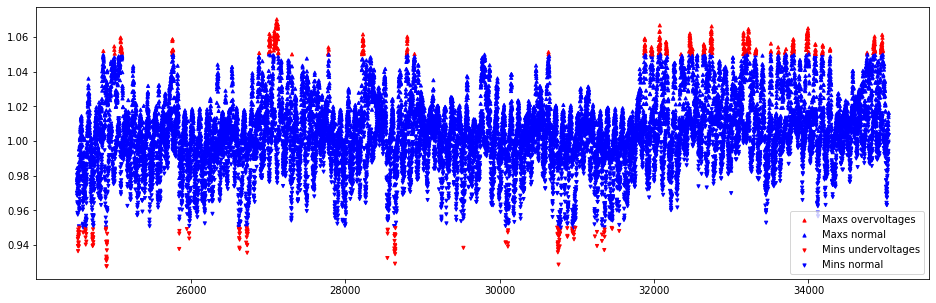
\includegraphics[width=.45\linewidth]{images/RL/before.png}
%     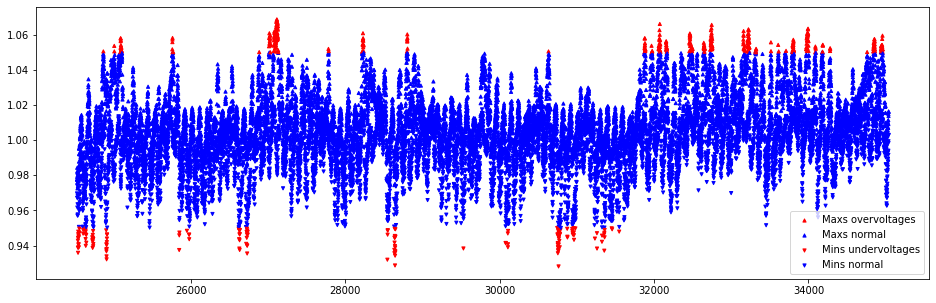
\includegraphics[width=.45\linewidth]{images/RL/after.png}
% \caption{Before (left) and after (right) the agent control. }

%  \end{figure}